\section{Rahmatul Ridha (1144124)}
\subsection{Teori}
\subsubsection{Soal No. 1}
\hfill \break
Apa itu fungsi library matplotlib?

\hfill \break
Matplotlib merupakan salah satu library Python 2D yang dapat menghasilkan plot dengan kualitas yang tinggi dalam berbagai format dan dapat digunakan di berbagai platform. Matplotlib berfungsi sebagai pembuat grafik di berbagai platform, seperti Python dan Jupyter. Grafik yang dibuat menggunakan Matplotlib bisa dibuat dalam berbagai bentuk, seperti grafik garis, batang, lingkaran, histogram, dan sebagainya.Matplotlib merupakan bagian dari paket inti SciPy dan ditawarkan dibawah lisensi BSD. Ini adalah library ilmiah pada python yang populer dan digunakan untuk menghasilkan visualisasi yang sederhana dan kuat. Anda dapat menggunakan kerangka kerja python untuk ilmu data dan menghasilkan grafik, chart, histogram, dan bentu atau gambar lain yang kreatuf tanpa perlu  khawatir menulis banyak baris kode. Matplotlib adalah library paling banyak digunakan oleh data science untuk menyajikan datanya ke dalam visual yang lebih baik.

\subsubsection{Soal No. 2}
\hfill \break
Jelaskan langkah-langkah membuat sumbu X dan Y di matplotlib!

\begin{enumerate}
	\item Pertama-tama import library Matplotlib.	
	\lstinputlisting[firstline=2, lastline=2]{src/6/1144124/1144124.py}
	
	\item Buat variable x dengan tujuan menampung list untuk sumbu X dan variabel y yang menampung list untuk sumbu Y.
	\lstinputlisting[firstline=4, lastline=5]{src/6/1144124/1144124.py}
	
	\item Panggil fungsi plot dan parameter pertama diisi dengan variabel x dan parameter kedua diisi dengan variabel y.
	\lstinputlisting[firstline=7, lastline=7]{src/6/1144124/1144124.py}	

	\item Setelah itu panggil plot yang tadi dengan memanggil fungsi show.
	\lstinputlisting[firstline=9, lastline=9]{src/6/1144124/1144124.py}
	
\end{enumerate}
\hfill \break
\textbf{Kode Program}

\lstinputlisting[caption = Kode program membuat diagram menggunakan Matplotlib., firstline=2, lastline=9]{src/6/1144124/1144124.py}

\hfill \break
\textbf{Hasil Compile}

\begin{figure}[H]
	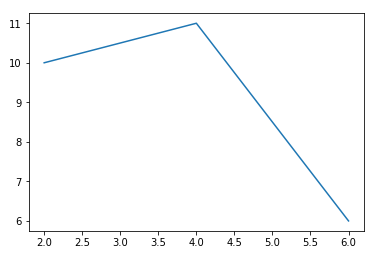
\includegraphics[width=7cm]{figures/6/1144124/2.png}
	\centering
	\caption{Hasil compile membuat diagram menggunakan Matplotlib.}
\end{figure}

\subsubsection{Soal No. 3}
\hfill \break
Jelaskan bagaimana perbedaan fungsi dan cara pakai untuk berbagai jenis(bar, histogram ,scatter ,line, dll) jenis plot di matplotlib!

\begin{enumerate}
	\item \textbf{Bar Graph}
	
	Perbedaan bar graph dengan jenis plot yang lain adalah bar graph menggunakan bar atau batang-batang untuk membandingkan data diantara berbagai kategori.
	
	\textbf{Kode Program}
	
	\lstinputlisting[caption = Kode program membuat bar graph menggunakan Matplotlib., firstline=2, lastline=9]{src/6/1144124/1144124.py}
	
	\textbf{Hasil Compile}
	
	\begin{figure}[H]
		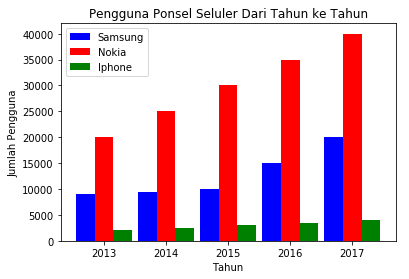
\includegraphics[width=7cm]{figures/6/1144124/bar.png}
		\centering
		\caption{Hasil compile membuat bar graph menggunakan Matplotlib.}
	\end{figure}
	
	\item \textbf{Histogram}
	
	Historigram adalah grafik yang menampilkan frekuensi data menggunakan batang, dimana angka dikelompokkan dalam rentang tertentu. Dengan kata lain, frekuensi setiap elemen data di dalam daftar ditunjukkan menggunakan histogram. Angka yang dikelompokkan dalam bentuk rentang tertentu disebut bins. Perbedaan histogram dengan jenis plot yang lain adalah histogram akan membuat plot, dimana plot yang akan dimunculkan merupakan gabungan dari beberapa data yang sudah dikelompokkan.
	
	\textbf{Kode Program}
	
	\lstinputlisting[caption = Kode program membuat histogram menggunakan Matplotlib., firstline=29, lastline=36]{src/6/1144124/1144124.py}
	
	\textbf{Hasil Compile}
	
	\begin{figure}[H]
		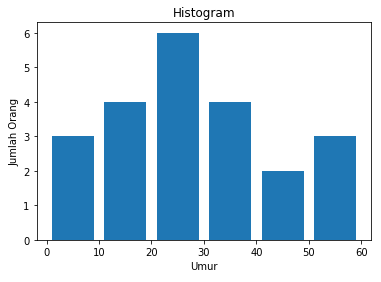
\includegraphics[width=7cm]{figures/6/1144124/histogram.png}
		\centering
		\caption{Hasil compile membuat histogram menggunakan Matplotlib.}
	\end{figure}
	
	\item \textbf{Scatter Plot}
	
	Scatter Plot adalah sebuah grafik yang menunjukkan hubungan antara dua set data, seperti hubungan antara umur dan tinggi. Perbedaan scatter plot dengan jenis plot lain adalah scatter plot berfungsi untuk menampilkan data sebagai kumpulan titik.
	
	\textbf{Kode Program}
	
	\lstinputlisting[caption = Kode program membuat scatter plot menggunakan Matplotlib., firstline=40, lastline=53]{src/6/1144124/1144124.py}
	
	\textbf{Hasil Compile}
	
	\begin{figure}[H]
		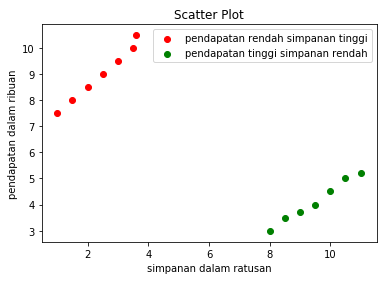
\includegraphics[width=7cm]{figures/6/1144124/scatter.png}
		\centering
		\caption{Hasil compile membuat scatter plot menggunakan Matplotlib.}
	\end{figure}
	
	\item \textbf{Area Plot}
	
	Perbedaan area plot dengan jenis plot lain adalah area plot dapat digunakan untuk melacak suatu perubahan dari waktu ke waktu untuk dua atau lebih kelompok yang terkait dan membentuk satu kategori secara keseluruhan.
	
	\textbf{Kode Program}
	
	\lstinputlisting[caption = Kode program membuat diagram menggunakan Matplotlib., firstline=57, lastline=76]{src/6/1144124/1144124.py}
	
	\textbf{Hasil Compile}
	
	\begin{figure}[H]
		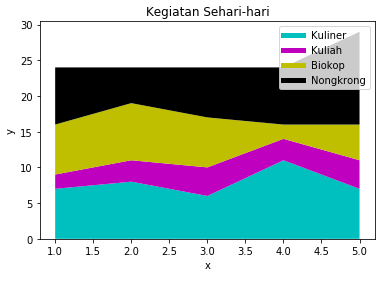
\includegraphics[width=7cm]{figures/6/1144124/area.png}
		\centering
		\caption{Hasil compile membuat diagram menggunakan Matplotlib.}
	\end{figure}
	
	\item \textbf{Pie Plot}
	
	Perbedaan pie plot dengan jenis plot lain adalah pie plot digunakan untuk menunjukkan data atau data proporsional dimana setiap potongan piee mewakili setiap kategori.
	
	\textbf{Kode Program}
	
	\lstinputlisting[caption = Kode program membuat Pie Plot menggunakan Matplotlib., firstline=80, lastline=101]{src/6/1144124/1144124.py}
	
	\textbf{Hasil Compile}
	
	\begin{figure}[H]
		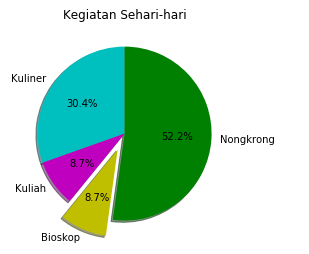
\includegraphics[width=6cm]{figures/6/1144124/pie.png}
		\centering
		\caption{Hasil compile untuk membuat Pie Plot menggunakan Matplotlib.}
	\end{figure}
	
	\item \textbf{Line Graph}
	
	Perbedaan line graph dengan jenis plot lain adalah line graph berfungsi untuk menapilkan diagram dalam bentuk garis.
	
	\textbf{Kode Program}
	
	\lstinputlisting[caption = Kode program untuk membuat diagram menggunakan Matplotlib., firstline=105, lastline=113]{src/6/1144124/1144124.py}
	
	\textbf{Hasil Compile}
	
	\begin{figure}[H]
		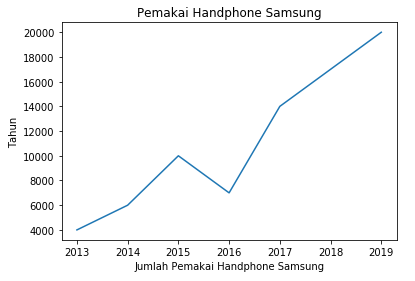
\includegraphics[width=7cm]{figures/6/1144124/line.png}
		\centering
		\caption{Hasil compile membuat diagram menggunakan Matplotlib.}
	\end{figure}
	
\end{enumerate}

\subsubsection{Soal No. 4}
\hfill \break
Jelaskan bagaimana cara menggunakan legend dan label serta kaitannya dengan fungsi tersebut!

\begin{enumerate}
	\item Untuk menggunakan legend yang didefinisikan ke parameter label di setiap fungsi plot. Parameter label digunakan untuk dapat memberikan label pada line sebagai pembeda antar line.
	
	\lstinputlisting[caption = Kode program yang menggunakan parameter label dengan Matplotlib., firstline=123, lastline=124]{src/6/1144124/1144124.py}
	
	\item Setelah itu panggil fungsi legend.
	
	\lstinputlisting[caption = Contoh kode program untuk memanggil fungsi legend dengan Matplotlib., firstline=128, lastline=128]{src/6/1144124/1144124.py}
\end{enumerate}

\hfill \break
\textbf{Kode Program}

\lstinputlisting[caption = Kode program membuat diagram menggunakan Matplotlib., firstline=117, lastline=130]{src/6/1144124/1144124.py}

\hfill \break
\textbf{Hasil Compile}

\begin{figure}[H]
	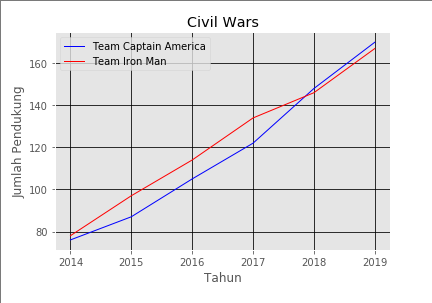
\includegraphics[width=7cm]{figures/6/1144124/4.png}
	\centering
	\caption{Hasil compile membuat diagram menggunakan Matplotlib.}
\end{figure}

\subsubsection{Soal No. 5}
\hfill \break
Jelaskan apa fungsi dari subplot di matplotlib, dan bagaimana cara kerja dari fungsi subplot, sertakan ilustrasi dan gambar sendiri dan apa parameternya jika ingin menggambar plot dengan 9 subplot di dalamnya!

\hfill \break
Subplot adalah fungsi yang membuat seolah-olah grafik kita sebagai sebuah elemen matrix dalam sebuah window. Fungsi Matplotlib subplot () yaitu dapat dipanggil untuk memplot dua atau lebih plot dalam satu gambar. Matplotlib mendukung semua jenis subplot termasuk 2 x 1 vertikal, 2 x 1 horizontal atau 2 x 2 kisi. Fungsi subplot didefinisikan sebelum fungsi plot grafik didefinisikan :
\begin{itemize}
  \item Banyaknya subplot didefinisikan dalam `m x n’ dengan `m’ adalah banyaknya beris subplot dan `n’ adalah banyaknya kolom subplot pada figure.
  \item Index subplot didefinisikan dalam `i’ yang merupakan urutan dari subplot.
  \item Dan juga dapat menggunakan berbagai fungsi plot yang ada pada library matlab.
\end{itemize}

\hfill \break
Cara kerja subplot, yaitu fungsi subplot memiliki parameter pertama adalah jumlah kolom, parameter kedua adalah jumlah baris, dan parameter ketiga adalah index plot keberapanya.

\hfill \break
\textbf{Kode Program}

\lstinputlisting[caption = Kode program membuat subplot menggunakan Matplotlib., firstline=134, lastline=146]{src/6/1144124/1144124.py}

\hfill \break
\textbf{Hasil Compile}

\begin{figure}[H]
	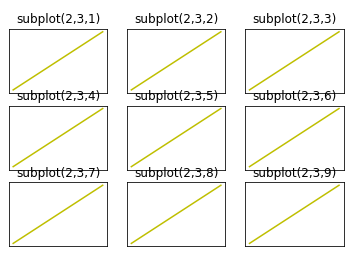
\includegraphics[width=7cm]{figures/6/1144124/subplot.png}
	\centering
	\caption{Hasil compile membuat subplot menggunakan Matplotlib.}
\end{figure}

\subsubsection{Soal No. 6}
\hfill \break
Sebutkan semua parameter color yang bisa digunakan (contoh:  m,c,r,k,...  dkk)!

Ini adalah fungsi do-nothing untuk memberi Anda bantuan tentang cara matplotlib menangani warna. Perintah yang mengambil argumen warna dapat menggunakan beberapa format untuk menentukan warna. Untuk warna bawaan dasar, Anda dapat menggunakan satu huruf.
\begin{itemize}
	\item 'b' (blue)
	\item 'g' (green)
	\item 'r' (red)
	\item 'c' (cyan)
	\item 'm' (magenta)
	\item 'y' (yellow)
	\item 'k' (black)
	\item 'w' (white)
\end{itemize}

\subsubsection{Soal No. 7}
\hfill \break
Jelaskan bagaimana cara kerja dari fungsi hist, sertakan ilustrasi dan gambar sendiri!

\hfill \break
Cara kerja dari fungsi hist adalah dimana fungsi hist akan menerima parameter yang telah diberikan, setelah itu fungsi hist akan disksekusi sesuai dengan parameter yang telah diberikan.

\hfill \break
\textbf{Kode Program}

\lstinputlisting[caption = Kode program membuat diagram menggunakan Matplotlib., firstline=150, lastline=157]{src/6/1144124/1144124.py}

\hfill \break
\textbf{Hasil Compile}

\begin{figure}[H]
	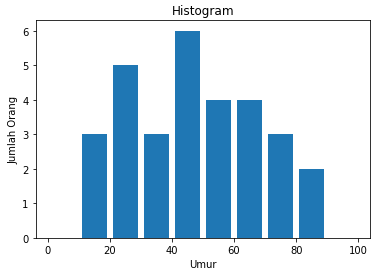
\includegraphics[width=7cm]{figures/6/1144124/7.png}
	\centering
	\caption{Hasil compile membuat diagram menggunakan Matplotlib.}
\end{figure}

\subsubsection{Soal No. 8}
\hfill \break
 Jelaskan lebih mendalam tentang parameter dari fungsi pie diantaranya labels, colors, startangle, shadow, explode, autopct!

 \begin{itemize}
 	\item labels : berfungsi untuk memberikan label di tiap persentase.
 	\item colors : berfungsi untuk memberikan warna di tiap persentase.
 	\item startangle : berfungsi untuk memutar plot sesuai dengan derajat yang ditentukan.
 	\item shadow : berfungsi untuk memberikan bayangan pada plot.
 	\item explode : berfungsi untuk memisahkan antar tiap potongan pie pada plot.
 	\item autopct : berfungsi untuk menentukan jumlah angka dibelakang koma.
 \end{itemize}

\subsection{Praktek}
\subsubsection{Soal No. 1}
\hfill \break
Buatlah librari fungsi (file terpisah/library dengan nama NPMbar.py) untuk plot dengan jumlah subplot adalah NPM mod 3 + 2!

\subsubsection{Soal No. 2}
\hfill \break
Buatlah librari fungsi (file terpisah/library dengan nama NPMscatter.py) untuk plot dengan jumlah subplot NPM mod 3 + 2!

\subsubsection{Soal No. 3}
\hfill \break
Buatlah librari fungsi (file terpisah/library dengan nama NPMpie.py) untuk plot dengan jumlah subplot NPM mod 3 + 2!

\subsubsection{Soal No. 4}
\hfill \break
Buatlah librari fungsi (file terpisah/library dengan nama NPMplot.py) untuk plot dengan jumlah subplot NPM mod 3 + 2


\subsection{Penanganan Error}
Tuliskan  peringatan  error  yang  didapat  dari  mengerjakan  praktek  keenam  ini, dan  jelaskan  cara  penanganan  error  tersebut. dan  Buatlah  satu  fungsi  yang menggunakan try except untuk menanggulangi error tersebut.
